\section{Catmull-Clark}

\subsection{Allgemein}

Der Catmull-Clark Algorithmus wurde 1978 von Edwin Catmull und James Clark entwickelt.
Er basiert auf bi-cubic uniform B-spline surfaces.
Der ursprüngliche Algorithmus war nur für Vierecksnetze definiert.
Hier wird eine erweiterte Form verwendet, die mit beliebiger Topologie umgehen kann.
Das neu erzeugte Netz ist immer ein Vierecksnetz.
Jedes n-Gon im Eingabenetz wird in n Quads
im Ausgabenetz umgewandelt.
Die Kontrollpunkte des Netzes werden durch Unterteilung approximiert.
Catmull-Clark erzeugt im Normalfall \(C^2\) Flächen,
an extraordinären Stellen mit Valence ungleich vier jedoch
nur \(C^1\).
\cite[S. 75ff]{Zorin.subdivcourse} \cite[S. 52ff]{Standford.24.07.2015}


\subsection{Unterteilungsregel}

Um ein Kontrollnetz nach Catmull-Clark zu unterteilen sind vier Schritte notwendig.
\begin{enumerate}
	\item Füge für jedes Polygon einen neuen Punkt hinzu (face point).
	\item Füge für jede Kante einen neuen Punkt hinzu (edge point).
	\item Berechne für jeden alten Kontrollpunkt die neue Position (original point).
	\item Verbinde die Punkte (face point, edge point, original point), sodass diese ein
	neues verfeinerten Netz erzeugen (face split).
\end{enumerate}

\autoref{fig:sd_catmull_mask} zeigt die Masken, mit denen die jeweiligen Punkte für ein Viereck berechnet werden können.
Im folgenden wird der allgemeinere Fall für beliebige Polygone beschrieben.
\begin{figure}
\centering
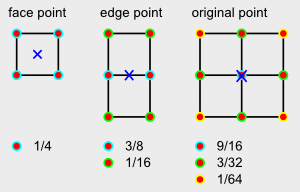
\includegraphics[width=0.5\textwidth]{content/media/sd_catmull_mask.png}
\caption{Catmull-Clark Maske für ein Viereck \cite{yoshihitoyagi.23.12.2015}}
\label{fig:sd_catmull_mask}
\end{figure}

\subsubsection*{Face Point}
Der face point berechnet sich als Mittelwert der Kontrollpunkte des Polygons.
Bei einem Viereck wie in \autoref{fig:sd_catmull_mask} hat somit jeder Kontrollpunkt
ein Gewicht von 1/4.

\subsubsection*{Edge Point}
Der edge point wird von den anliegenden Polygone beeinflusst.
Dieser errechnet sich aus dem Durchschnitt der zwei benachbarten Face Points und den
beiden Kontrollpunkten der Kante.

\subsubsection*{Original Point}
Jeder original point wird aktualisiert.
Die Berechnung wird folgendermaßen durchgeführt:\\
\(
new\_point=(Q/n) + (2R/n) + (S*(n-3)/n)\\
n:\ Valence\\
Q:\ Durchschnitt\ der\ umliegenden\ face\ points\\
R:\ Durchscnitt\ aller\ umliegenden\ Mittelpunkte\ der\ Ecken\ (!=\ edge\ point)\\
S:\ priginal\ point
\)

\subsubsection*{Face Split}
Nun sind alle notwendigen Punkte berechnet.
Die Punkte müssen durch Kanten zu gültigen Quads zusammengesetz werden.
Ein Quad besteht aus den 4 Ecken:
\begin{itemize}
 \item Original Point
 \item Edge Point 1
 \item Face Point
 \item Edge Point 2
\end{itemize}
Für jedes Polygon mit n Ecken entstehen n Quads.
\cite{rosettacode.23.12.2015}
\cite{rorydriscoll.23.12.2015}
\cite{yoshihitoyagi.23.12.2015}

\subsection{Boundary}

Für boundary cases können die Koeffizienten für kubische Splines verwendet werden.
Diese führen zu akzeptablen Ergebnissen, garantieren formal jedoch keine \(C^1\) Stetigkeit mehr. \cite[S. 75f]{Zorin.subdivcourse}
\autoref{fig:sd_catmull_boundary} zeigt die Gewichtung für Boundaries.
Der edge point wird durch den Mittelwert der Ecken berechnet.
Um den neuen original point zu berechnen, wird die rechte Maske aus \autoref{fig:sd_catmull_boundary}
verwendet.

\begin{figure}
\centering
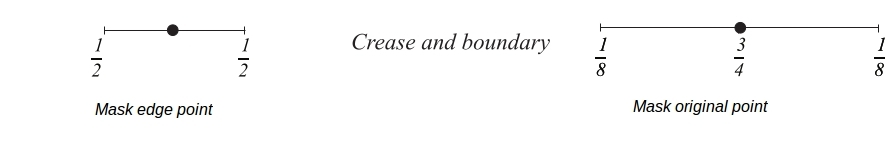
\includegraphics[width=1.0\textwidth]{content/media/sd_catmull_boundary.jpg}
\caption{Catmull-Clark Crease/Boundary \cite[S. 76]{Zorin.subdivcourse}}
\label{fig:sd_catmull_boundary}
\end{figure}



